\documentclass[compress]{beamer}
\usepackage{ifthen,verbatim}

\newcommand{\isnote}{}
\xdefinecolor{lightyellow}{rgb}{1.,1.,0.25}
\xdefinecolor{darkblue}{rgb}{0.1,0.1,0.7}

%% Uncomment this to get annotations
%% \def\notes{\addtocounter{page}{-1}
%%            \renewcommand{\isnote}{*}
%% 	   \beamertemplateshadingbackground{lightyellow}{white}
%%            \begin{frame}
%%            \frametitle{Notes for the previous page (page \insertpagenumber)}
%%            \itemize}
%% \def\endnotes{\enditemize
%% 	      \end{frame}
%%               \beamertemplateshadingbackground{white}{white}
%%               \renewcommand{\isnote}{}}

%% Uncomment this to not get annotations
\def\notes{\comment}
\def\endnotes{\endcomment}

\setbeamertemplate{navigation symbols}{}
\setbeamertemplate{headline}{\mbox{ } \hfill
\begin{minipage}{5.5 cm}
\vspace{-0.75 cm} \small
\end{minipage} \hfill
\begin{minipage}{4.5 cm}
\vspace{-0.75 cm} \small
\begin{flushright}
\ifthenelse{\equal{\insertpagenumber}{1}}{}{Jim Pivarski \hspace{0.2 cm} \insertpagenumber\isnote/\pageref{numpages}}
\end{flushright}
\end{minipage}\mbox{\hspace{0.2 cm}}\includegraphics[height=1 cm]{../cmslogo} \hspace{0.1 cm} \includegraphics[height=1 cm]{../tamulogo} \hspace{0.01 cm} \vspace{-1.05 cm}}

\newcommand{\s}[1]{{\mbox{\scriptsize #1}}}

\begin{document}
\begin{frame}
\vfill
\begin{center}
\textcolor{darkblue}{\Large Brief Update on A\&M Work}

\vfill
\begin{columns}
\column{0.3\linewidth}
\begin{center}
\large
Jim Pivarski

Aysen Tatarinov

Vadim Khotilovich

Alexei Safonov
\end{center}
\end{columns}

\begin{columns}
\column{0.3\linewidth}
\begin{center}
\scriptsize
{\it Texas A\&M University}
\end{center}
\end{columns}

\vfill
16 August, 2010

\end{center}
\end{frame}

%% \begin{notes}
%% \item This is the annotated version of my talk.
%% \item If you want the version that I am presenting, download the one
%% labeled ``slides'' on Indico (or just ignore these yellow pages).
%% \item The annotated version is provided for extra detail and a written
%% record of comments that I intend to make orally.
%% \item Yellow notes refer to the content on the {\it previous} page.
%% \item All other slides are identical for the two versions.
%% \end{notes}

\small

\begin{frame}
\frametitle{Since last time}
\begin{columns}
\column{0.6\linewidth}
\begin{itemize}
\item Settled on a baseline set of cuts
\begin{itemize}\setlength{\itemsep}{0.1 cm}
\item TrackerMuons with $N_\s{segments} \ge 2$ yield the same purity
  as GlobalMuons
\item it is essential that the segments in the count are arbitrated
\item even with the cut, TrackerMuons have a higher and easier-to-
  understand reconstruction efficiency for prompt muons
\item \textcolor{darkblue}{new:} by removing unnecessary additional
  cuts, TrackerMuons now have the same acceptance as GlobalMuons for
  highly displaced $\mu$-groups (plot on the right)
\end{itemize}
\item Starting to look at the new data
\end{itemize}

\column{0.5\linewidth}
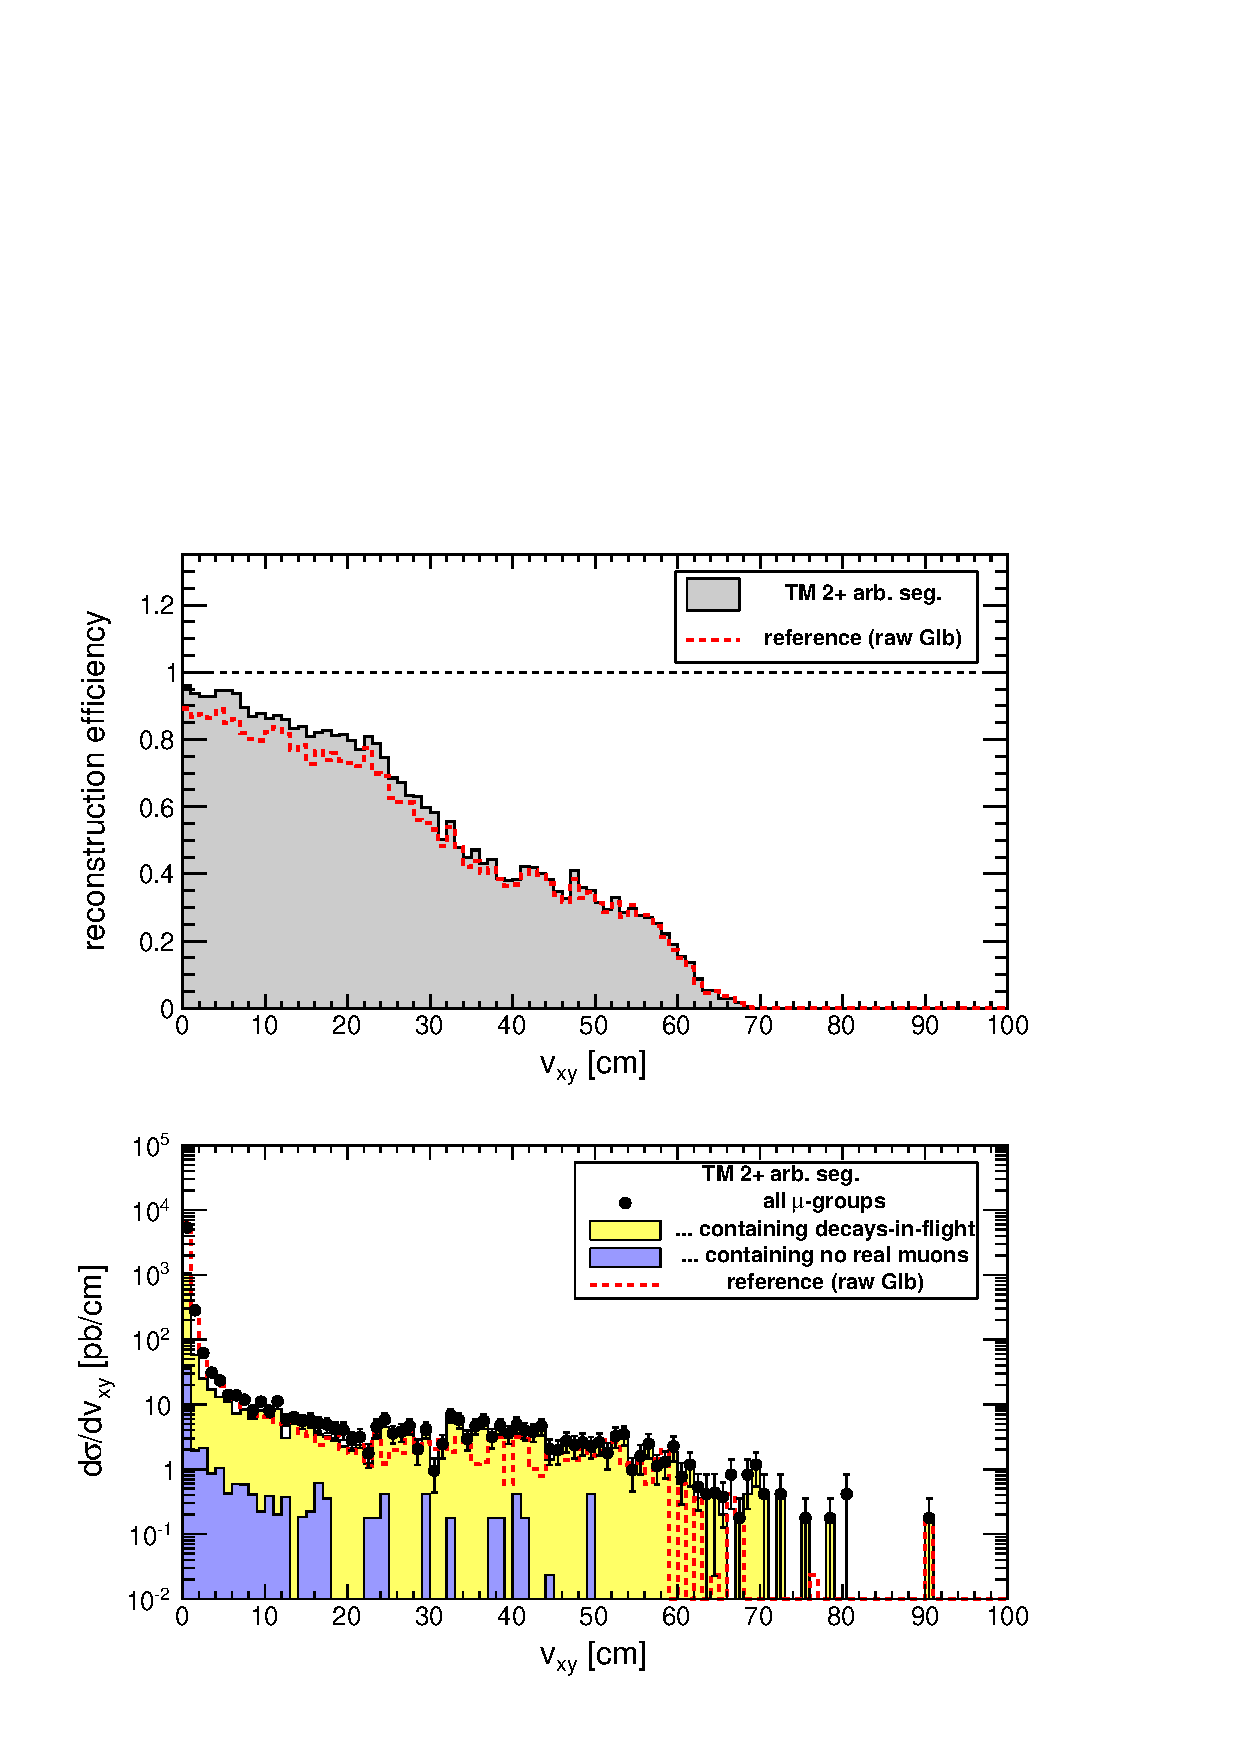
\includegraphics[width=\linewidth]{dispvert_TrackerSegMatch2.pdf}
\end{columns}
\end{frame}

\begin{frame}
\frametitle{Single $\mu$-group comparison}

\begin{itemize}
\item Opposite-sign groups of TrackerMuons with $N_\s{segments} \ge 2$, HLT\_Mu9, and $pT_1 > 11$~GeV/$c$ compared to InclusiveMu5\_Pt*
\item Prompt $J/\psi$ and $\psi(2S)$ are missing (understood)
\item $\omega \to \mu\mu$ is not in the Monte Carlo?  What about low-mass rise?
\end{itemize}

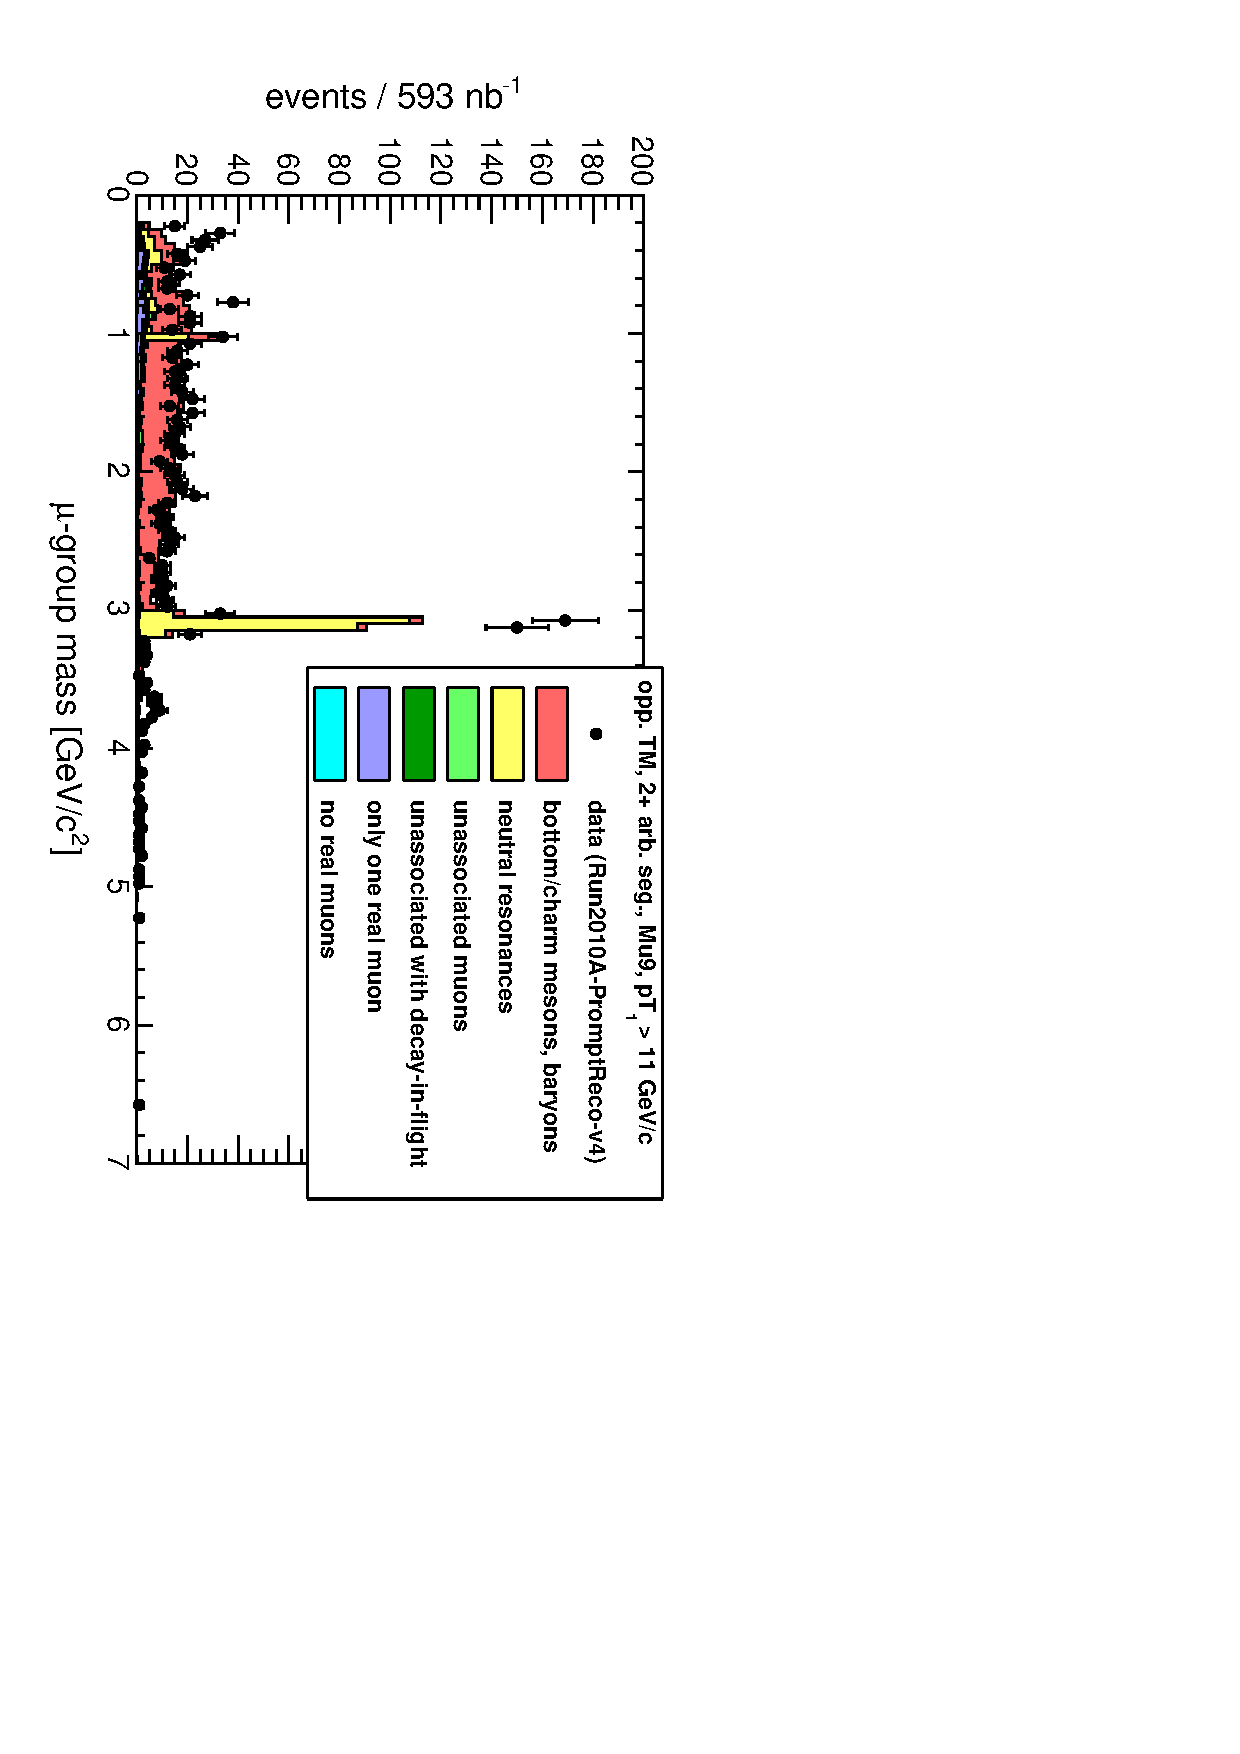
\includegraphics[height=\linewidth, angle=90]{Mu9_mass_general.pdf}
\end{frame}

\begin{frame}
\frametitle{Next steps (conclusions slide)}
\begin{itemize}\setlength{\itemsep}{0.25 cm}
\item Compare data and MC starting at the lowest levels of
  reconstruction (track-segment matching) and make sure everything is
  okay up to high level (kinematics)
\begin{itemize}
\item for example, the low-mass rise needs to be understood, but if
  the discrepancy is due to something at a deeper level, the best way
  to find it is to methodically check everything from the bottom up
\end{itemize}

\item Trigger efficiency studies

\item Estimating backgrounds from data
\end{itemize}
\label{numpages}
\end{frame}

\begin{frame}
\frametitle{Backup 1: close-ups of mass}

\begin{columns}
\column{0.5\linewidth}
Note: these two are from HLT\_Mu5 with $pT_1 > 7$~GeV/$c$

\vspace{0.25 cm}
{\scriptsize $\omega \to \mu\mu$ is in real data, but not MC}

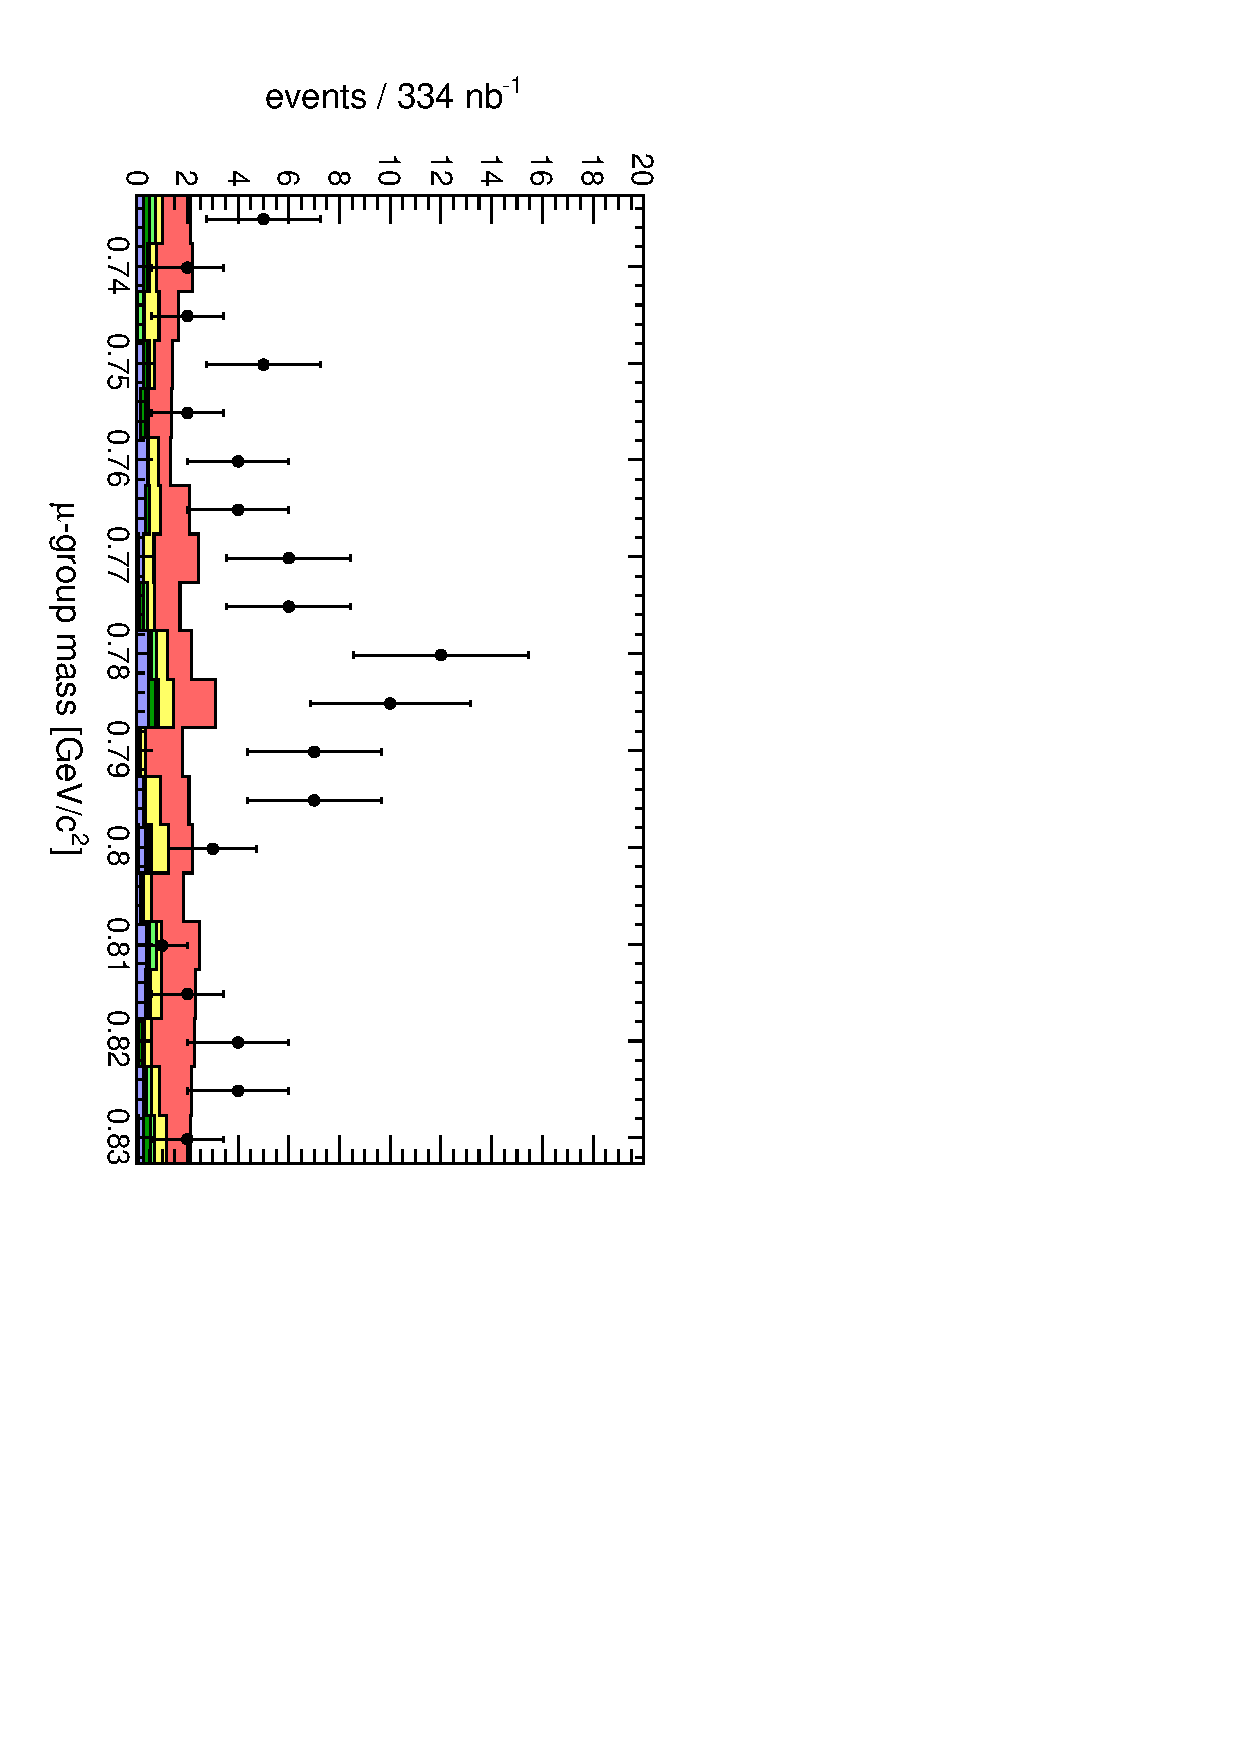
\includegraphics[height=\linewidth, angle=90]{Mu5_mass_omg.pdf}

\vspace{0.1 cm}
{\scriptsize $\phi \to \mu\mu$ is in MC, but perhaps too few}

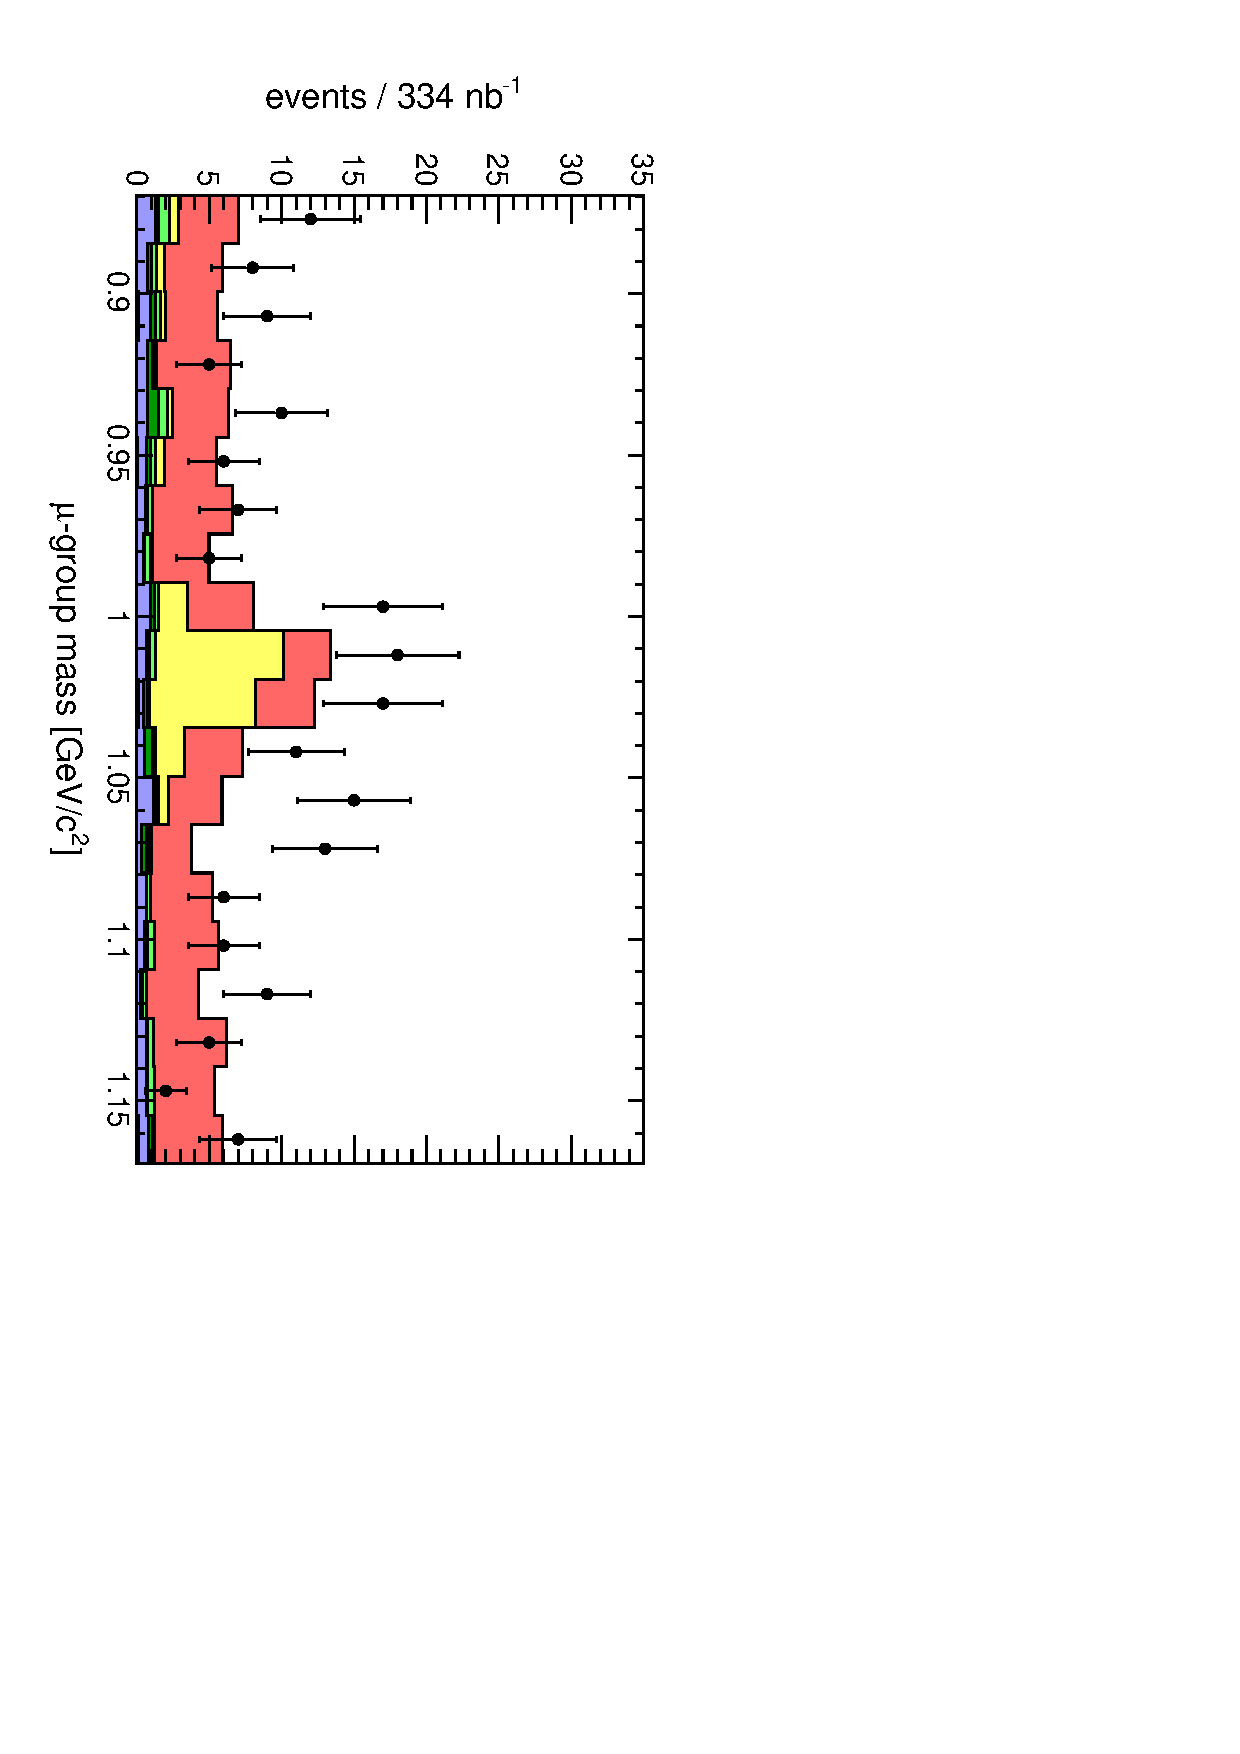
\includegraphics[height=\linewidth, angle=90]{Mu5_mass_phi.pdf}

\column{0.5\linewidth}
This is a $p_T$ distribution of $\mu$-groups in a mass window around the $J/\psi$

\vspace{0.1 cm}
{\scriptsize It's the low-momentum part that's missing, and I know
  that prompt $J/\psi$ are not included in the InclusiveMu5\_Pt*}

\vspace{0.25 cm}
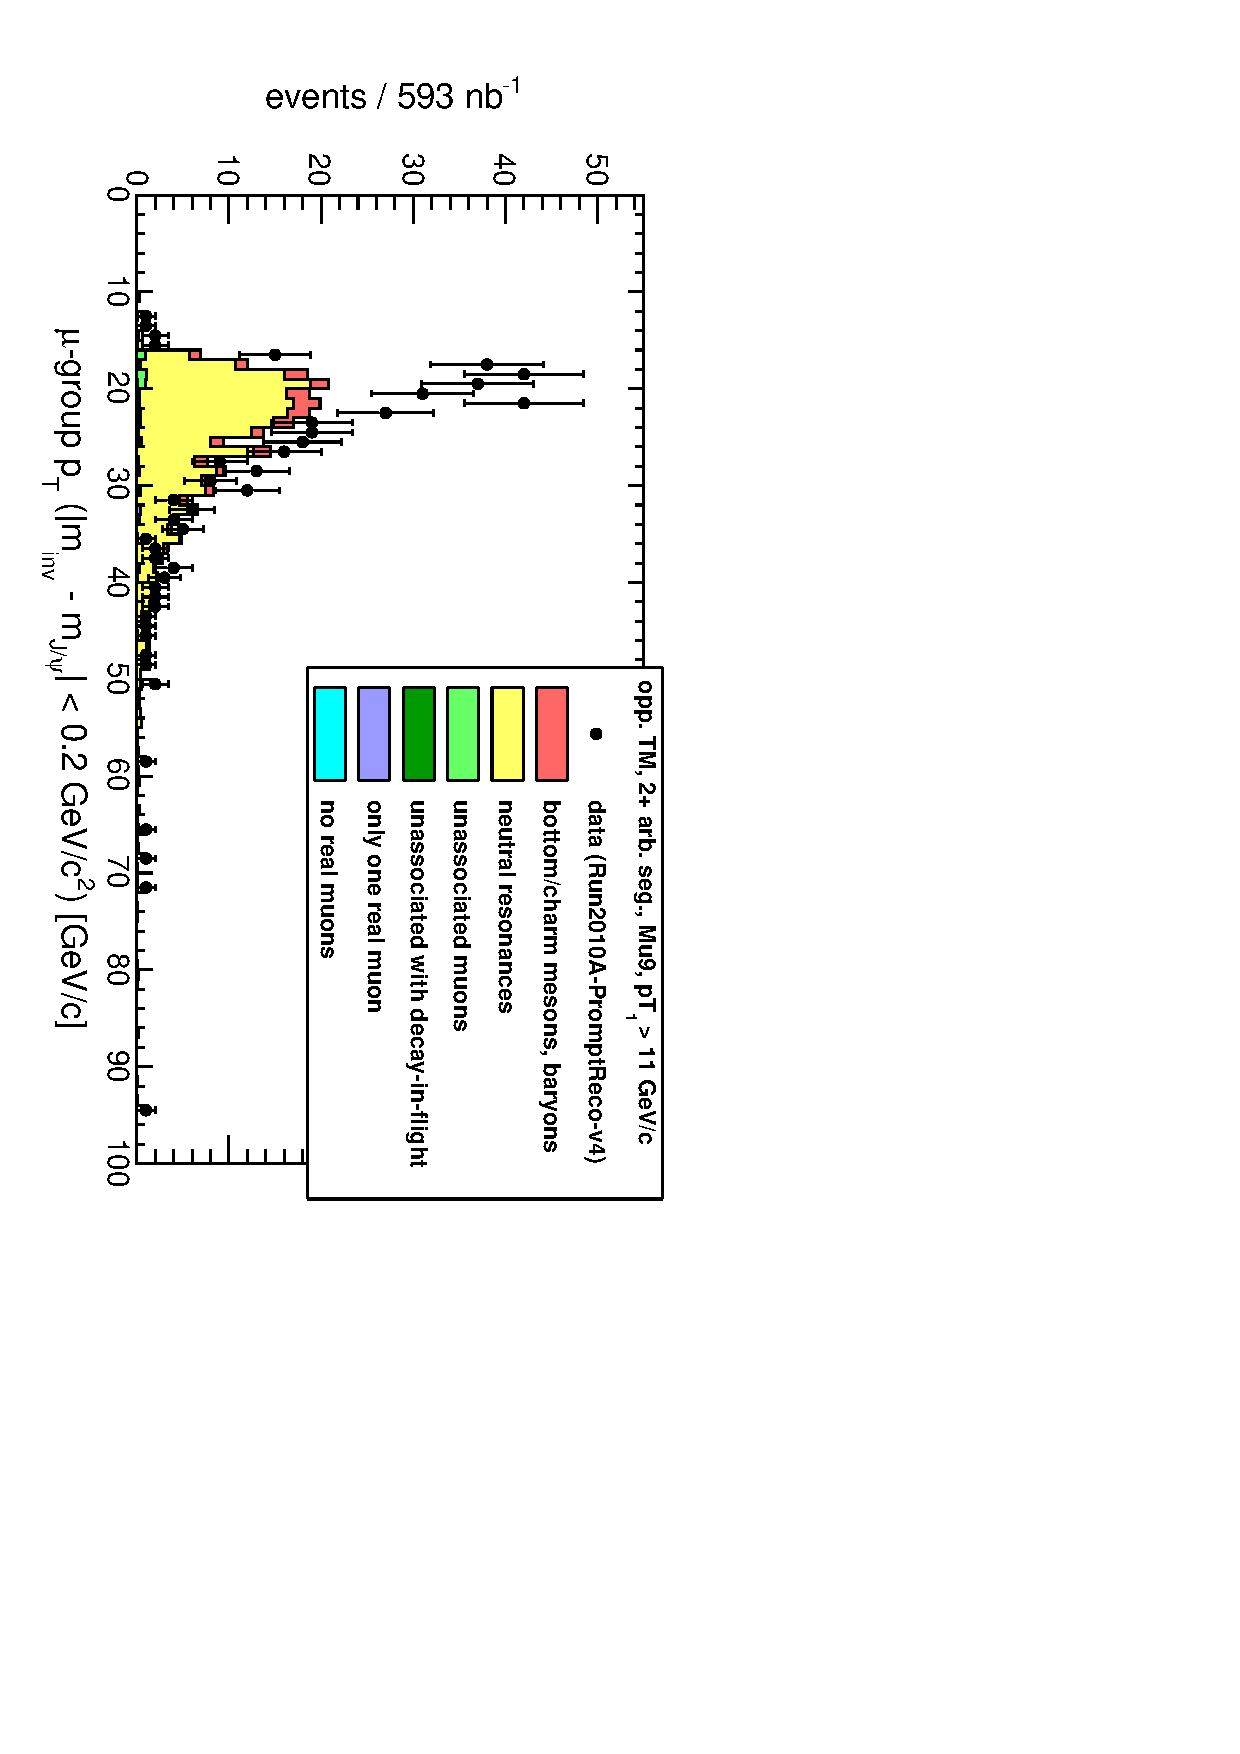
\includegraphics[height=\linewidth, angle=90]{Mu9_pt_jpsi.pdf}
\end{columns}
\end{frame}

\begin{frame}
\frametitle{Backup 2: low-mass event}

The $\mathcal{O}(100)$ $m_\s{inv} < 0.4$~GeV/$c^2$ events in data but not MC are
good-looking di-muons (this one has $m_\s{inv} < 0.25$~GeV/$c^2$)

\vspace{0.25 cm}
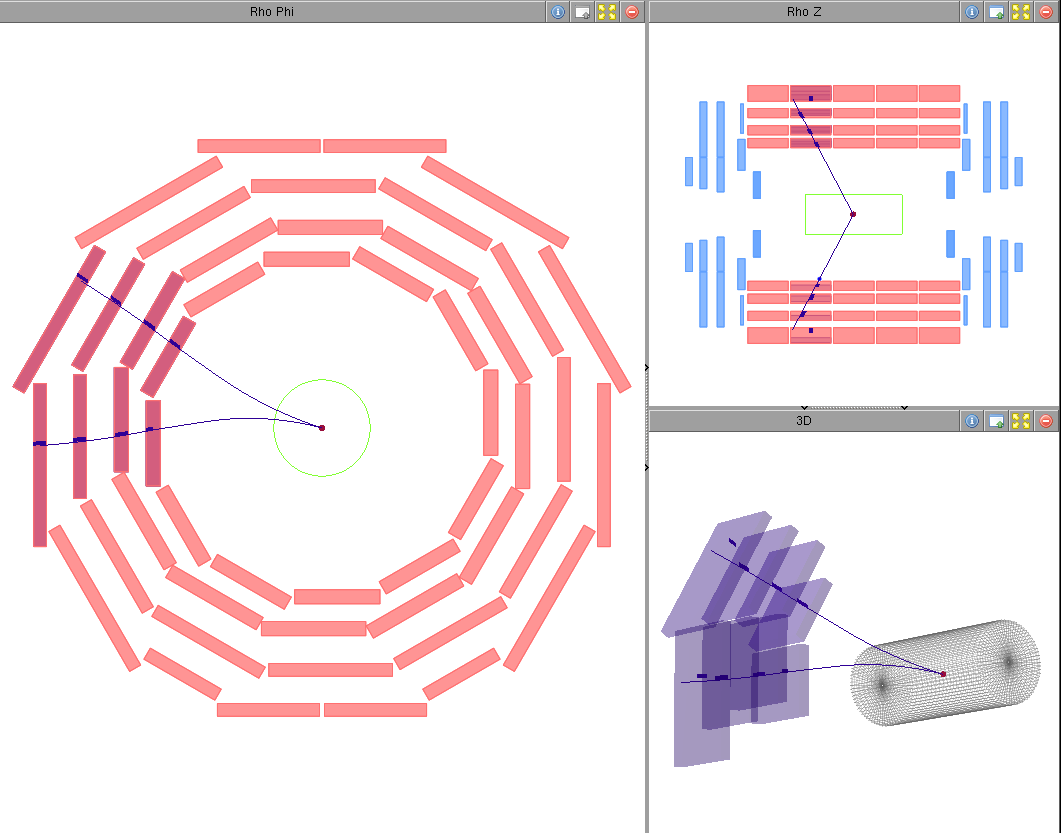
\includegraphics[width=0.9\linewidth]{low-mass_perfectly-normal_2.png}
\end{frame}

\begin{frame}
\frametitle{Backup 3: cuts}
\begin{itemize}
\item Run/LS selection: good tracking, muons, and trigger, selected by
  runregparse.py and luminosity calculated by lumiCalc.py

\item Event-level:
\begin{itemize}\setlength{\itemsep}{0.1 cm}
\item HLT\_Mu9 (or HLT\_Mu5, correcting for prescale)
\item leading track $p_T > 11$~GeV/$c$ (or 7) and $|\eta| < 2.1$
\item at least one primary vertex with $|z| < 24$~cm (hn-cms-PO7TeV)
\item filter out scraping (Collisions2010Recipes)
\end{itemize}

\item Muon tracks:
\begin{itemize}\setlength{\itemsep}{0.1 cm}
\item $p_T > 5$~GeV/$c$, $|\eta| < 2.4$
\item TrackerMuons with $N_\s{segments} \ge 2$ (arbitrated)
\item all default cuts inherited
\end{itemize}

\item Muon-group ``closeness'' definition:
\begin{itemize}\setlength{\itemsep}{0.1 cm}
\item ($m_\s{pair} < 5$~GeV/$c^2$ {\bf and} $P_\s{vertex} > 1\%$) {\bf or} $\Delta R < 0.1$
\item pairs must be oppositely charged
\end{itemize}
\end{itemize}
\end{frame}

\begin{frame}
\frametitle{From last time: $N_\s{segments}$ cut}

\begin{itemize}
\item Requiring at least 2 {\it fully arbitrated} segments in TrackerMuons recovers purity of GlobalMuons
\end{itemize}

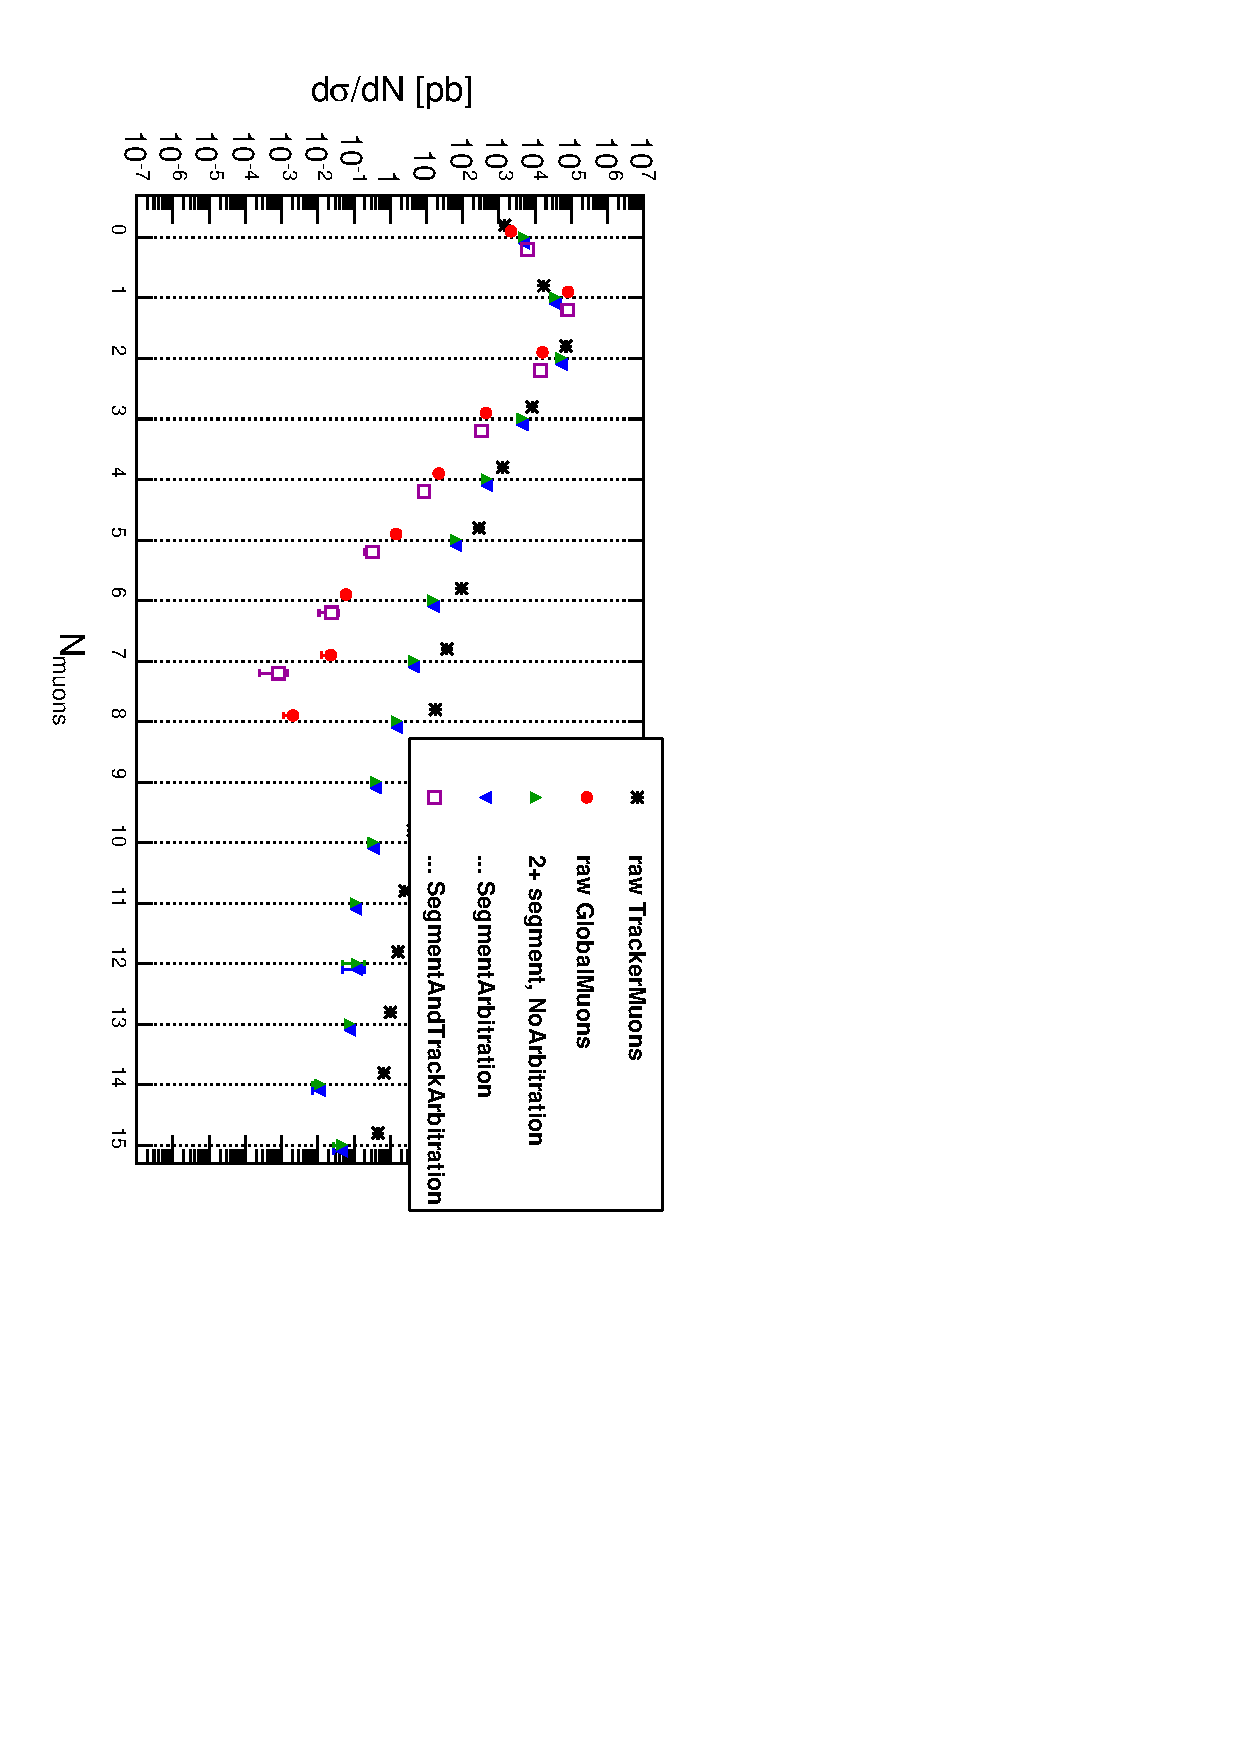
\includegraphics[height=\linewidth, angle=90]{tracks_lastpage_allreal.pdf}
\end{frame}

\begin{frame}
\frametitle{From last time: $N_\s{segments}$ cut}

\begin{itemize}
\item We see that we usually get the {\it right} number of muons
\item GlobalMuons and TrackerMuons + cut have the same backgrounds
\end{itemize}

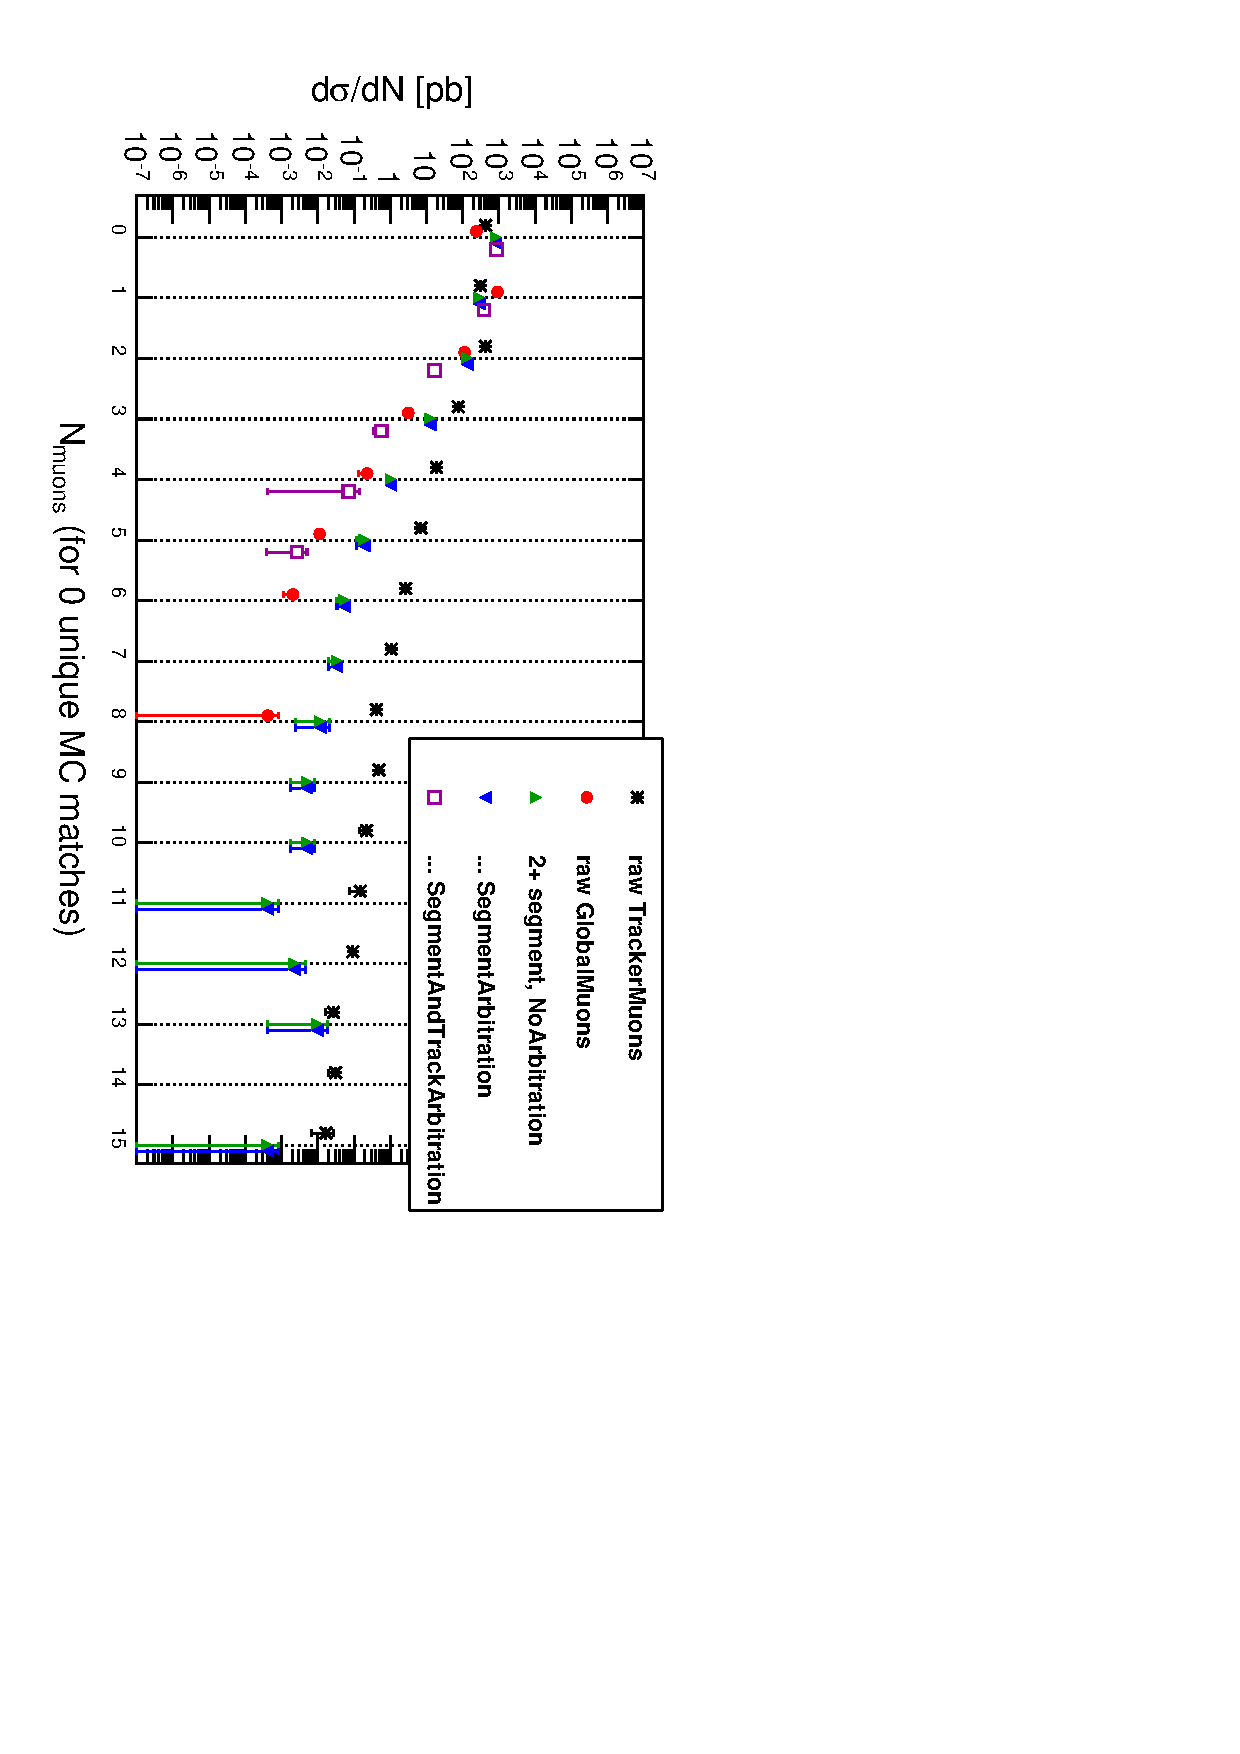
\includegraphics[height=0.49\linewidth, angle=90]{tracks_lastpage_0real.pdf}
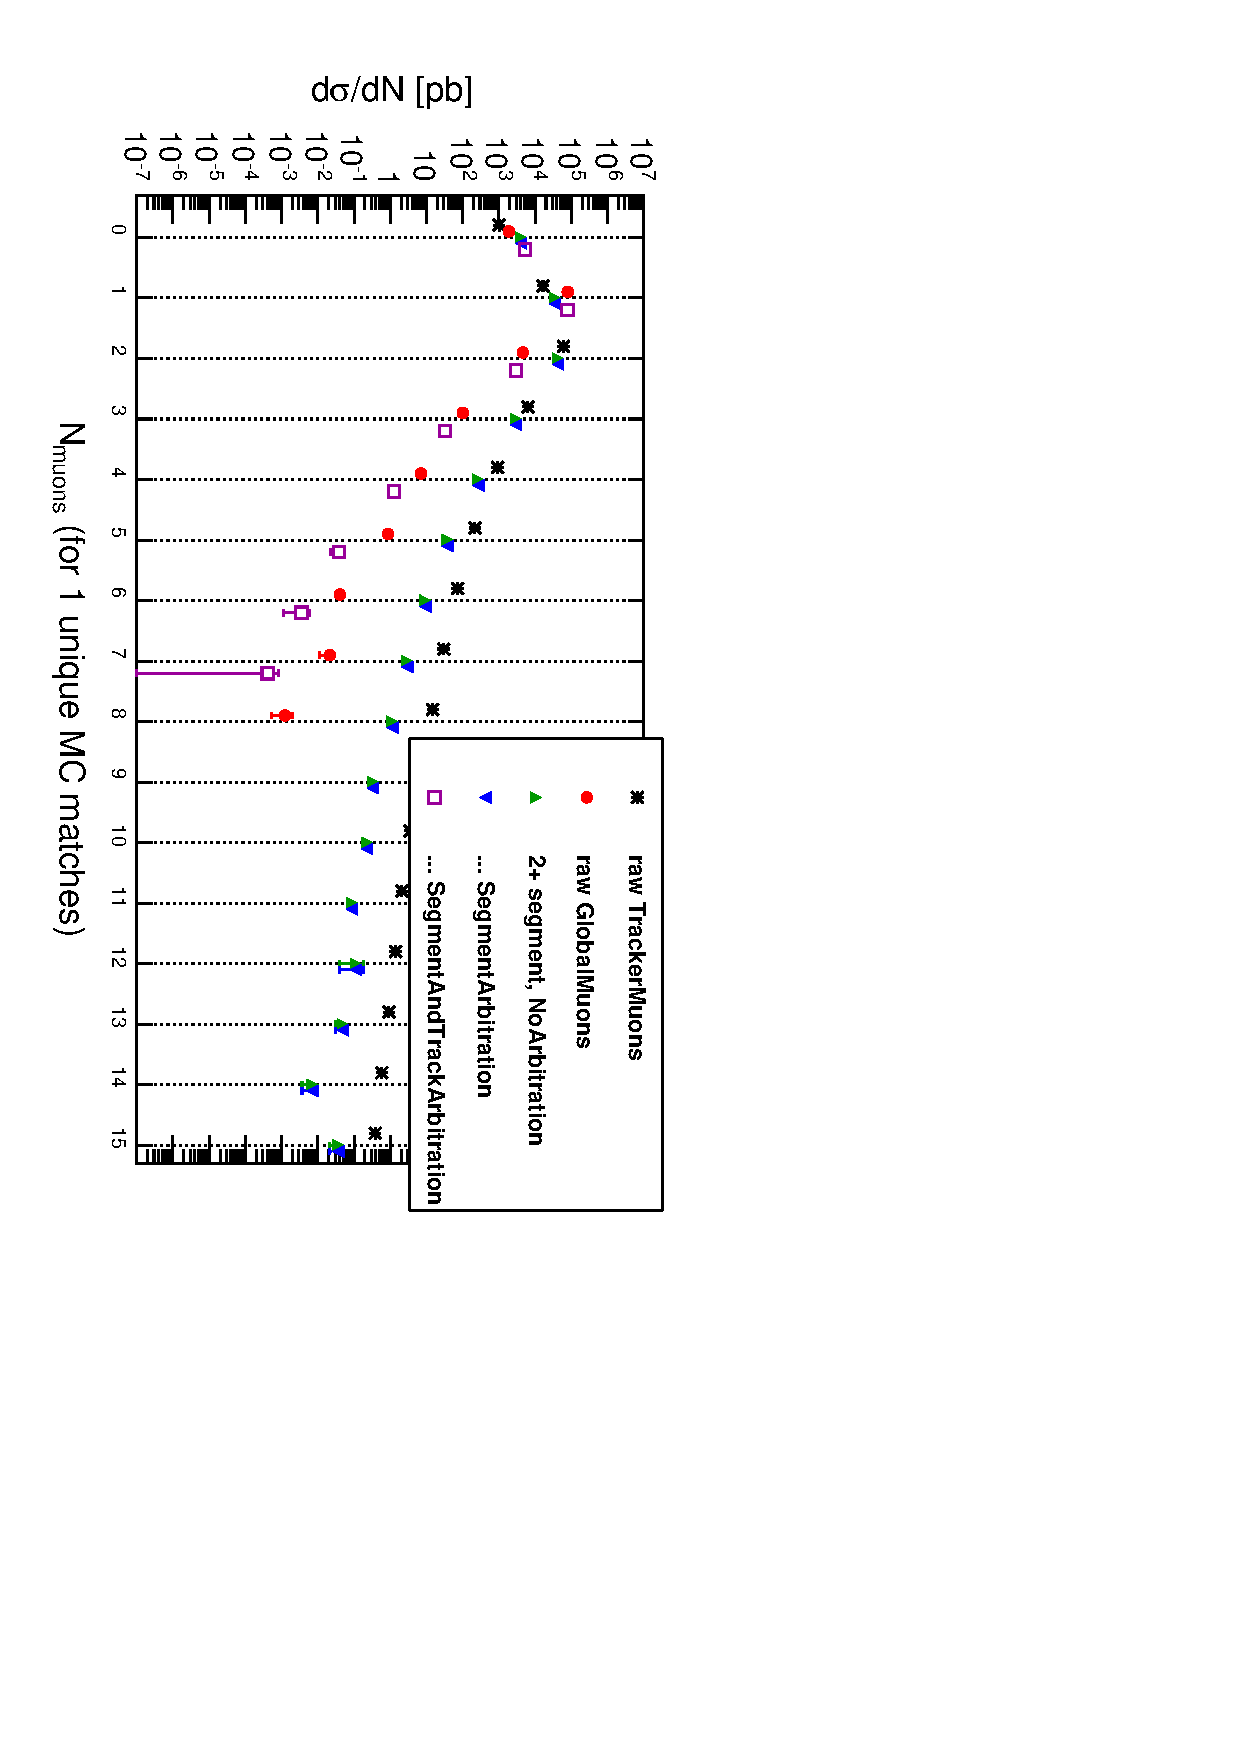
\includegraphics[height=0.49\linewidth, angle=90]{tracks_lastpage_1real.pdf}

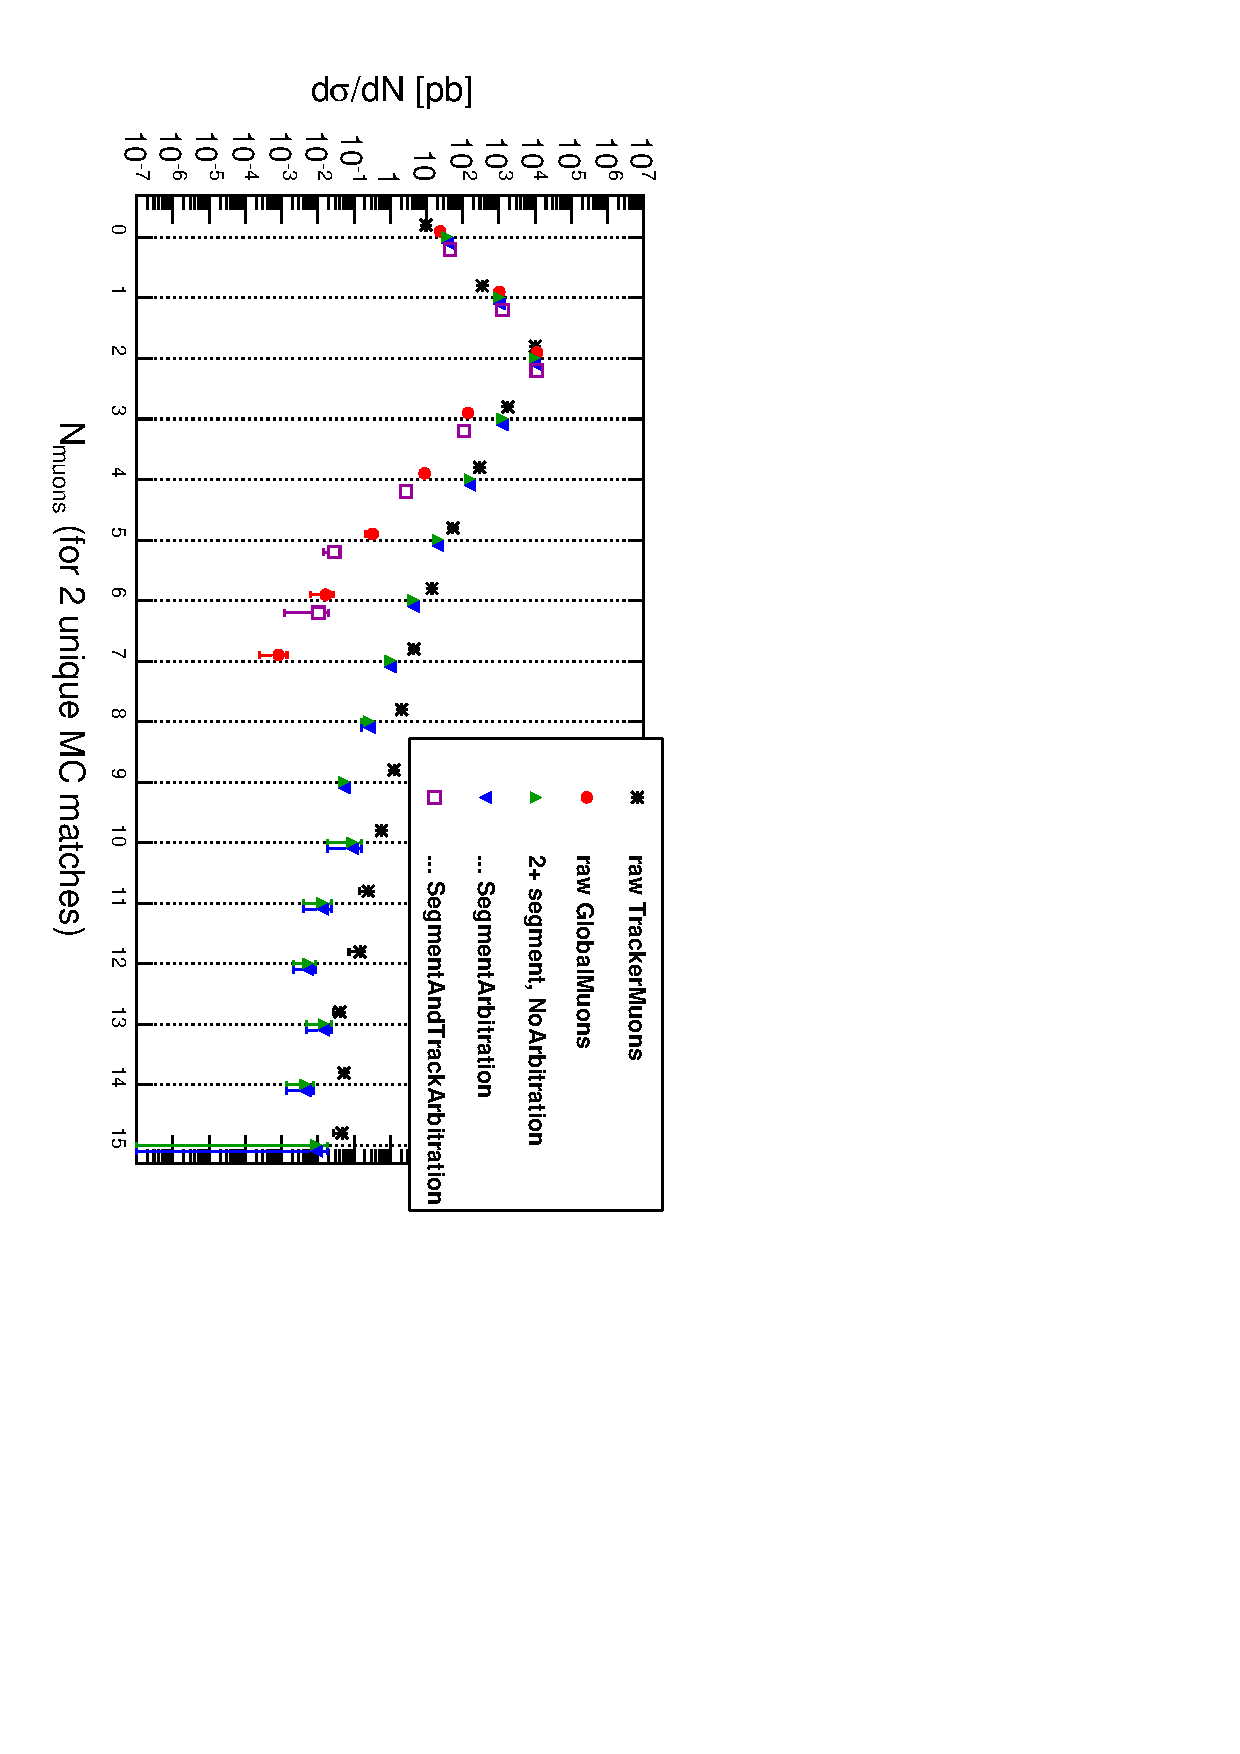
\includegraphics[height=0.49\linewidth, angle=90]{tracks_lastpage_2real.pdf}
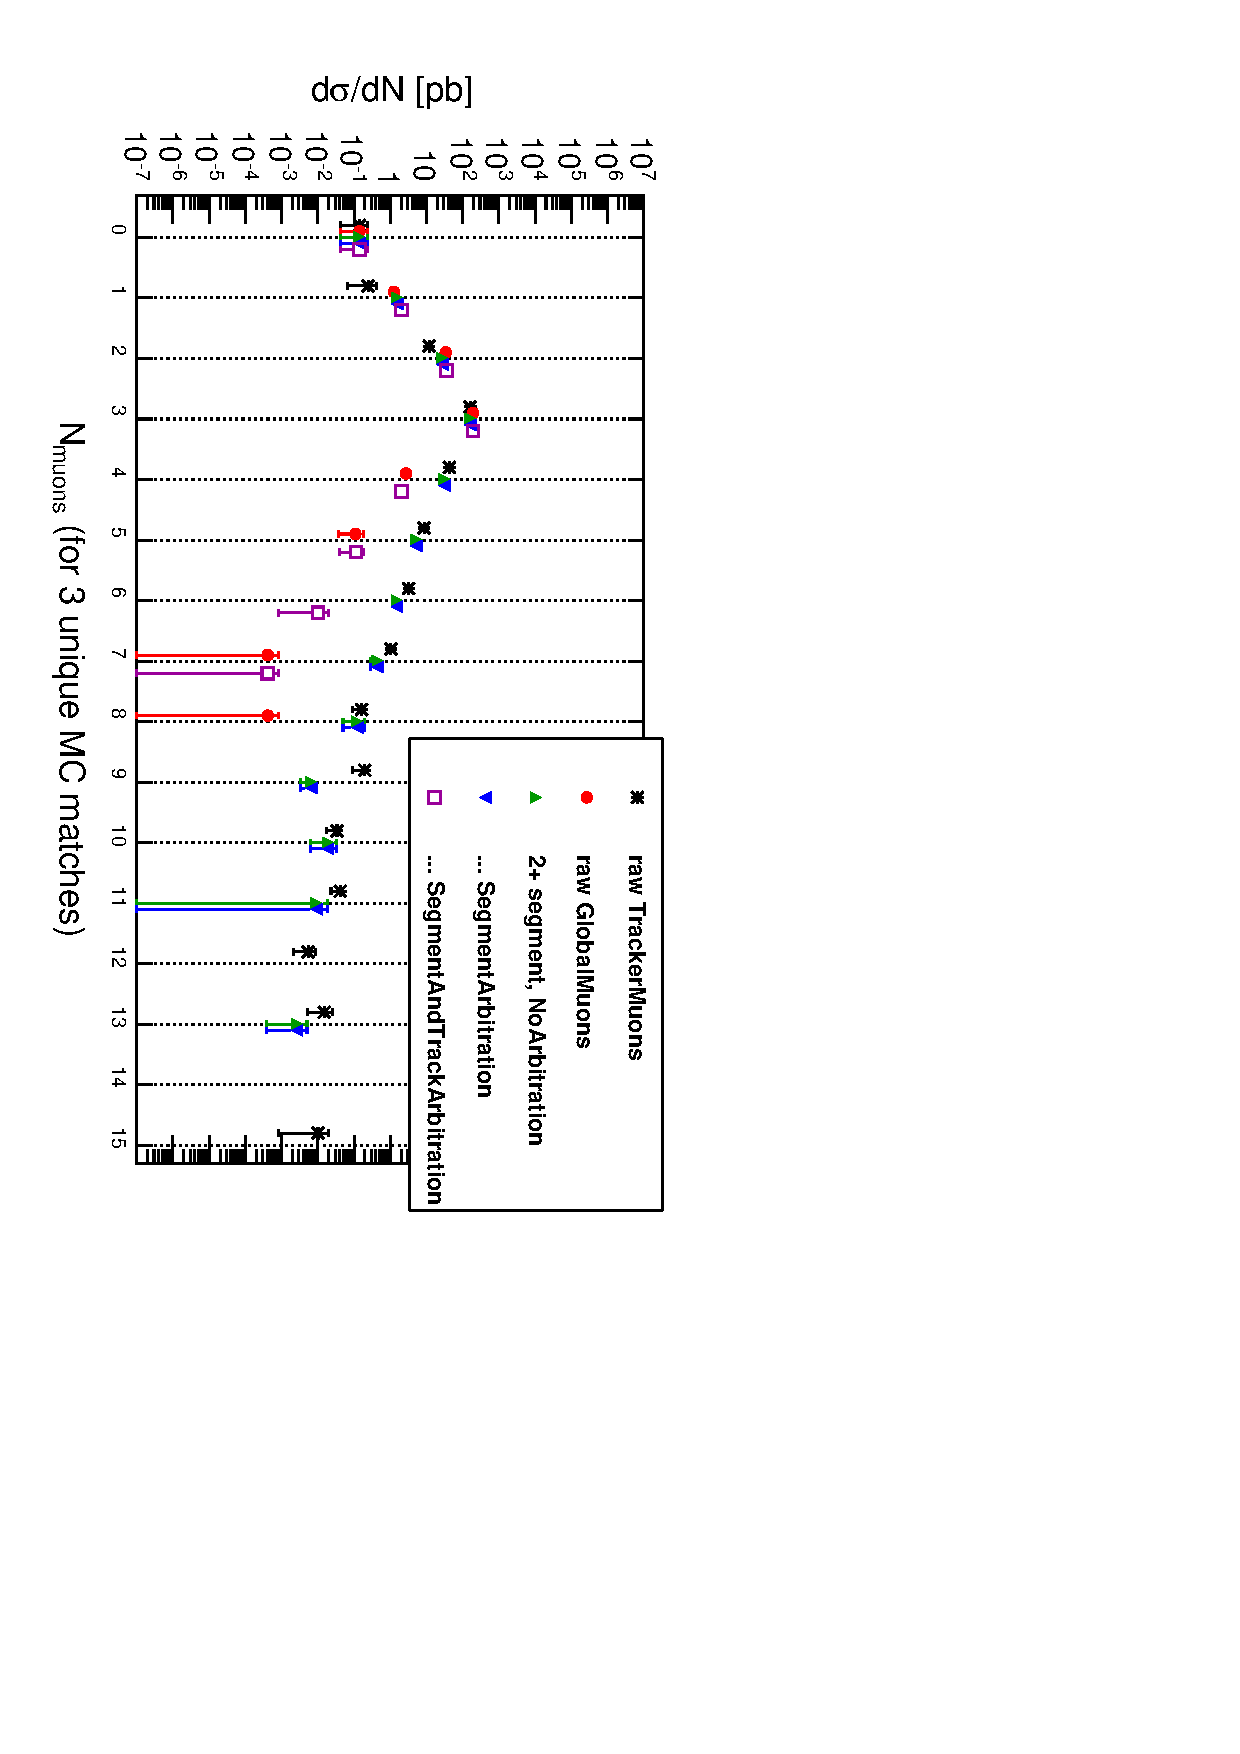
\includegraphics[height=0.49\linewidth, angle=90]{tracks_lastpage_3real.pdf}
\end{frame}

\begin{frame}
\frametitle{From last time: efficiency of cut}
\begin{itemize}
\item Efficiency versus $\Delta \phi = \phi_{\mu^+} - \phi_{\mu^-}$ in barrel (left) and endcap (right)
\item Top: GlobalMuons (barrel dependency not fully understood)
\item Bottom: TrackerMuons with arbitrated $N_\s{segments} \ge 2$
\end{itemize}

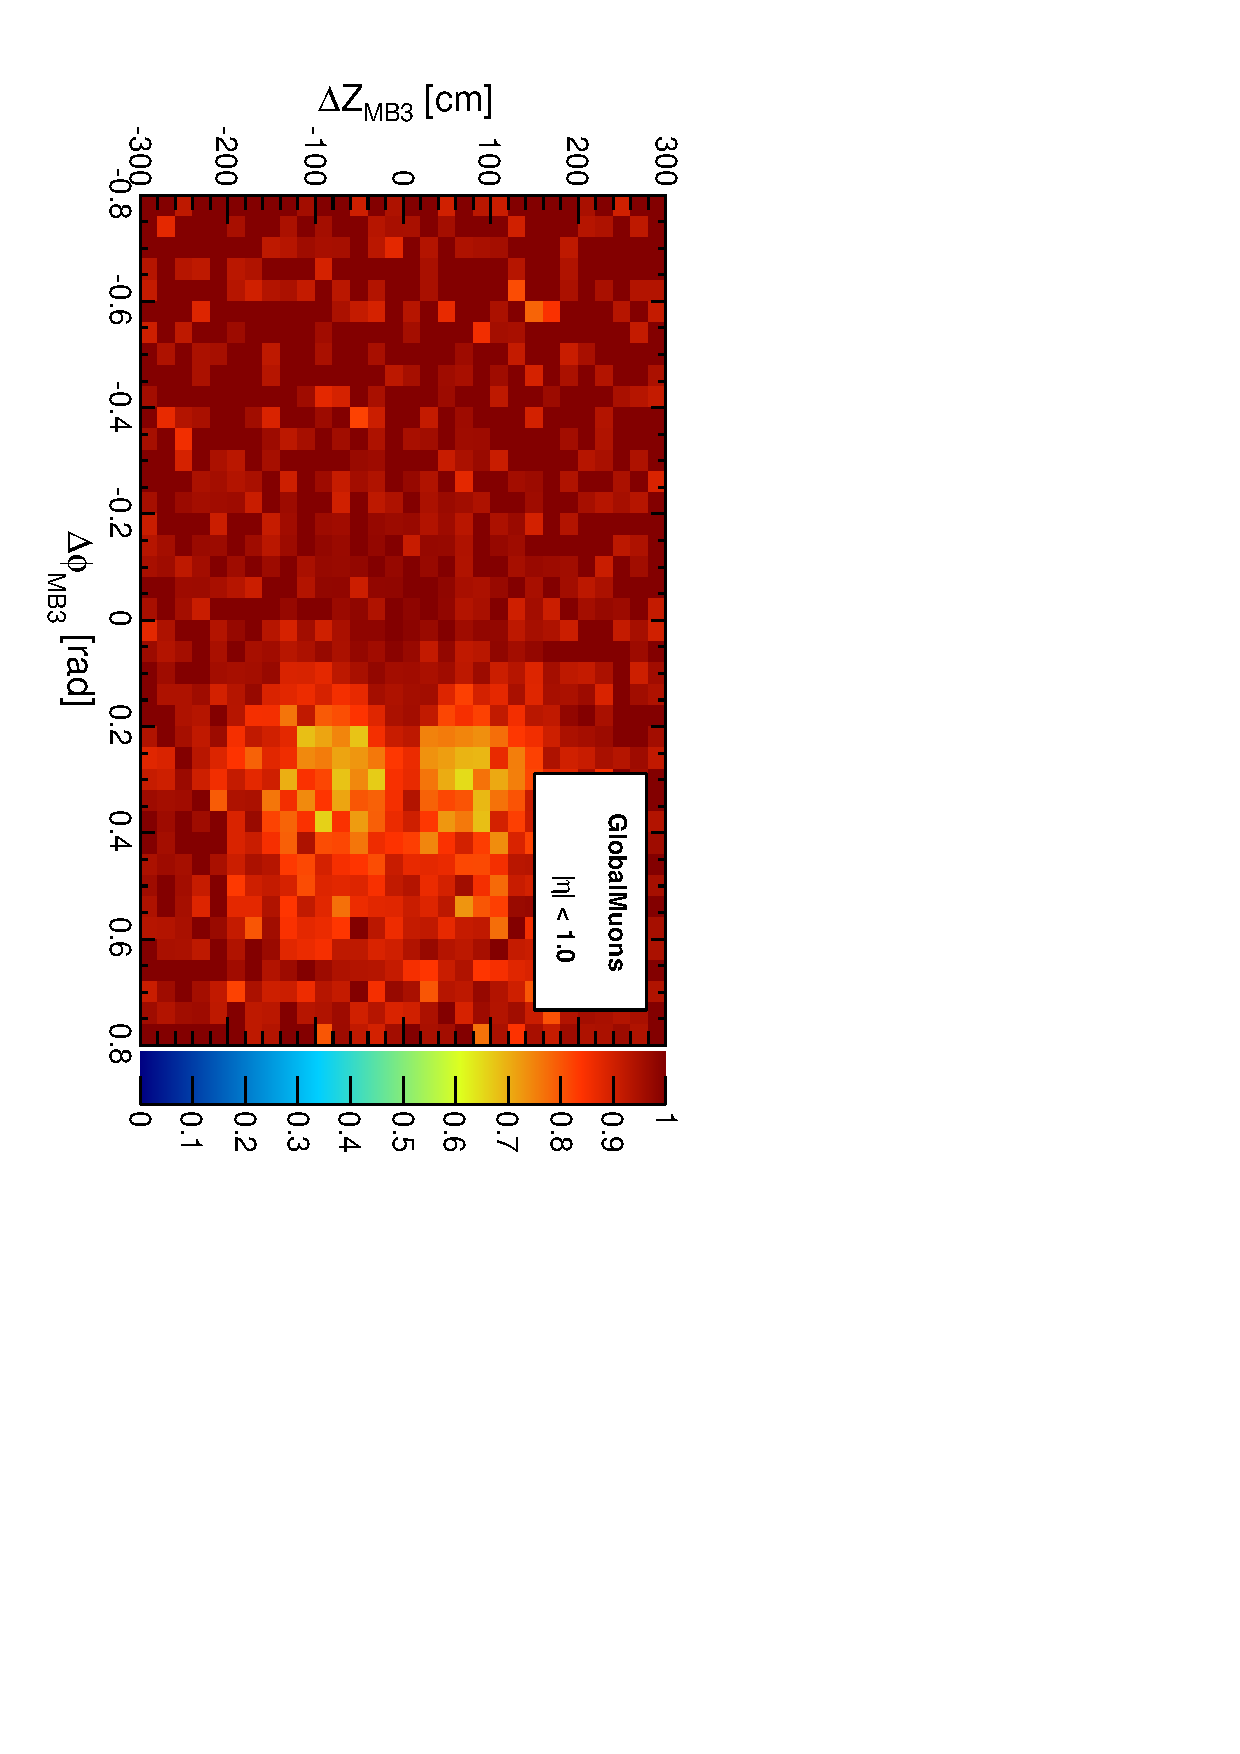
\includegraphics[height=0.49\linewidth, angle=90]{mb3_GlobalMuons.pdf}
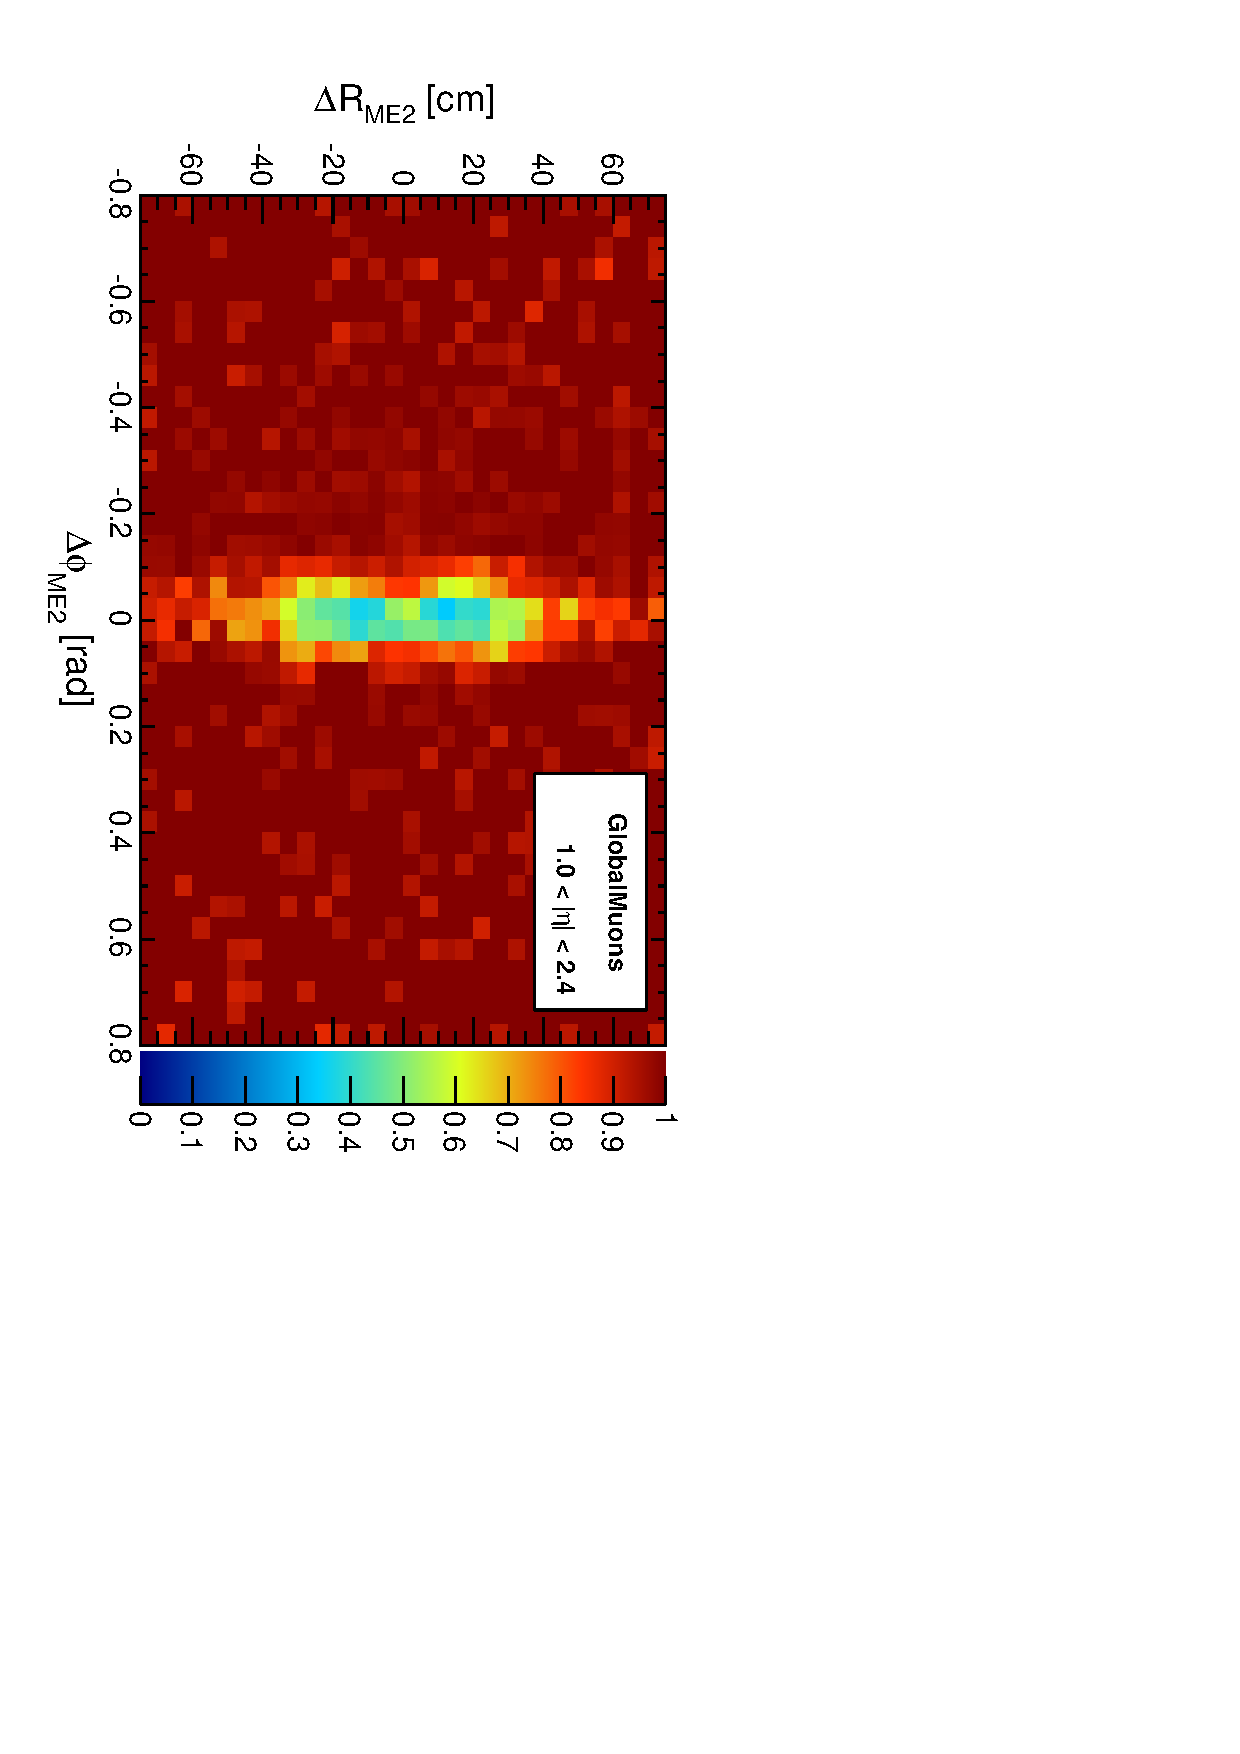
\includegraphics[height=0.49\linewidth, angle=90]{me2_GlobalMuons.pdf}

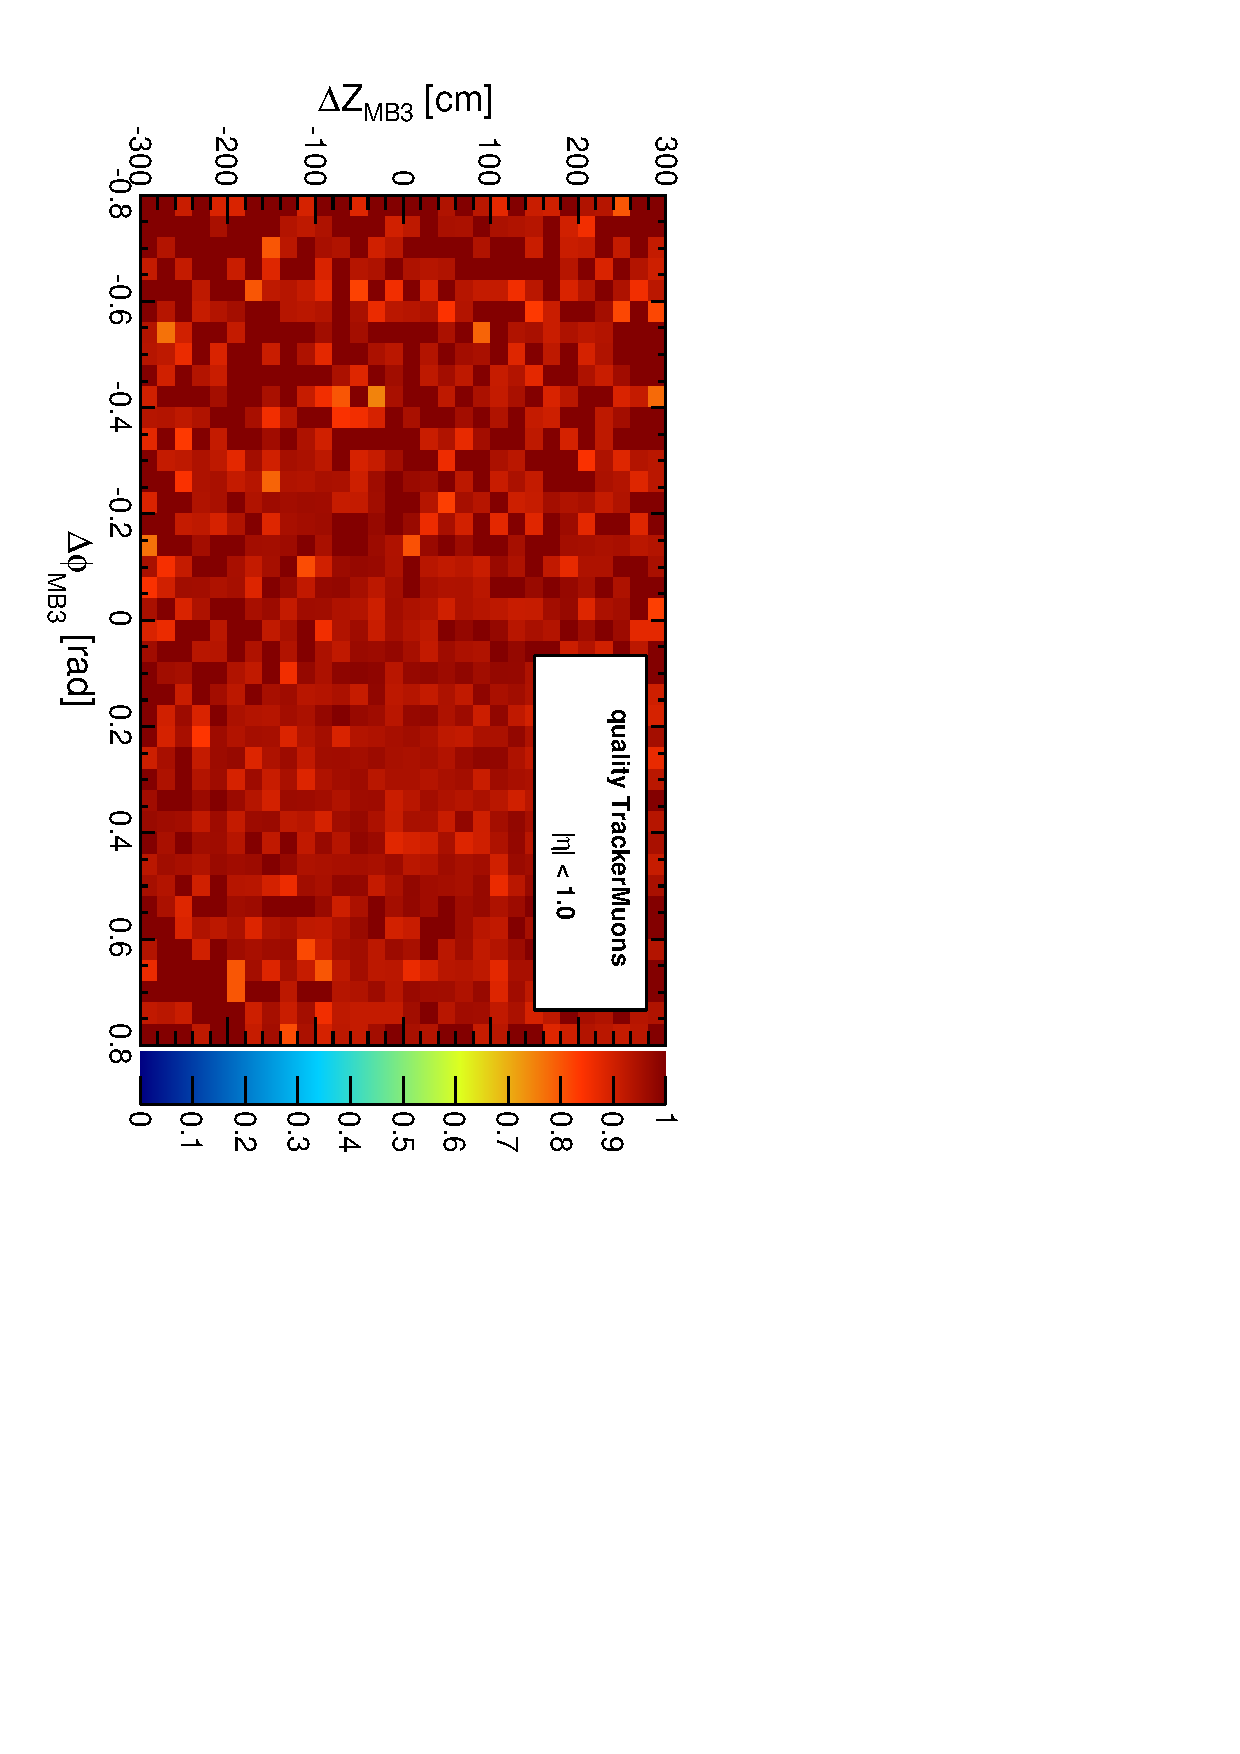
\includegraphics[height=0.49\linewidth, angle=90]{mb3_PlainTrackerMuon.pdf}
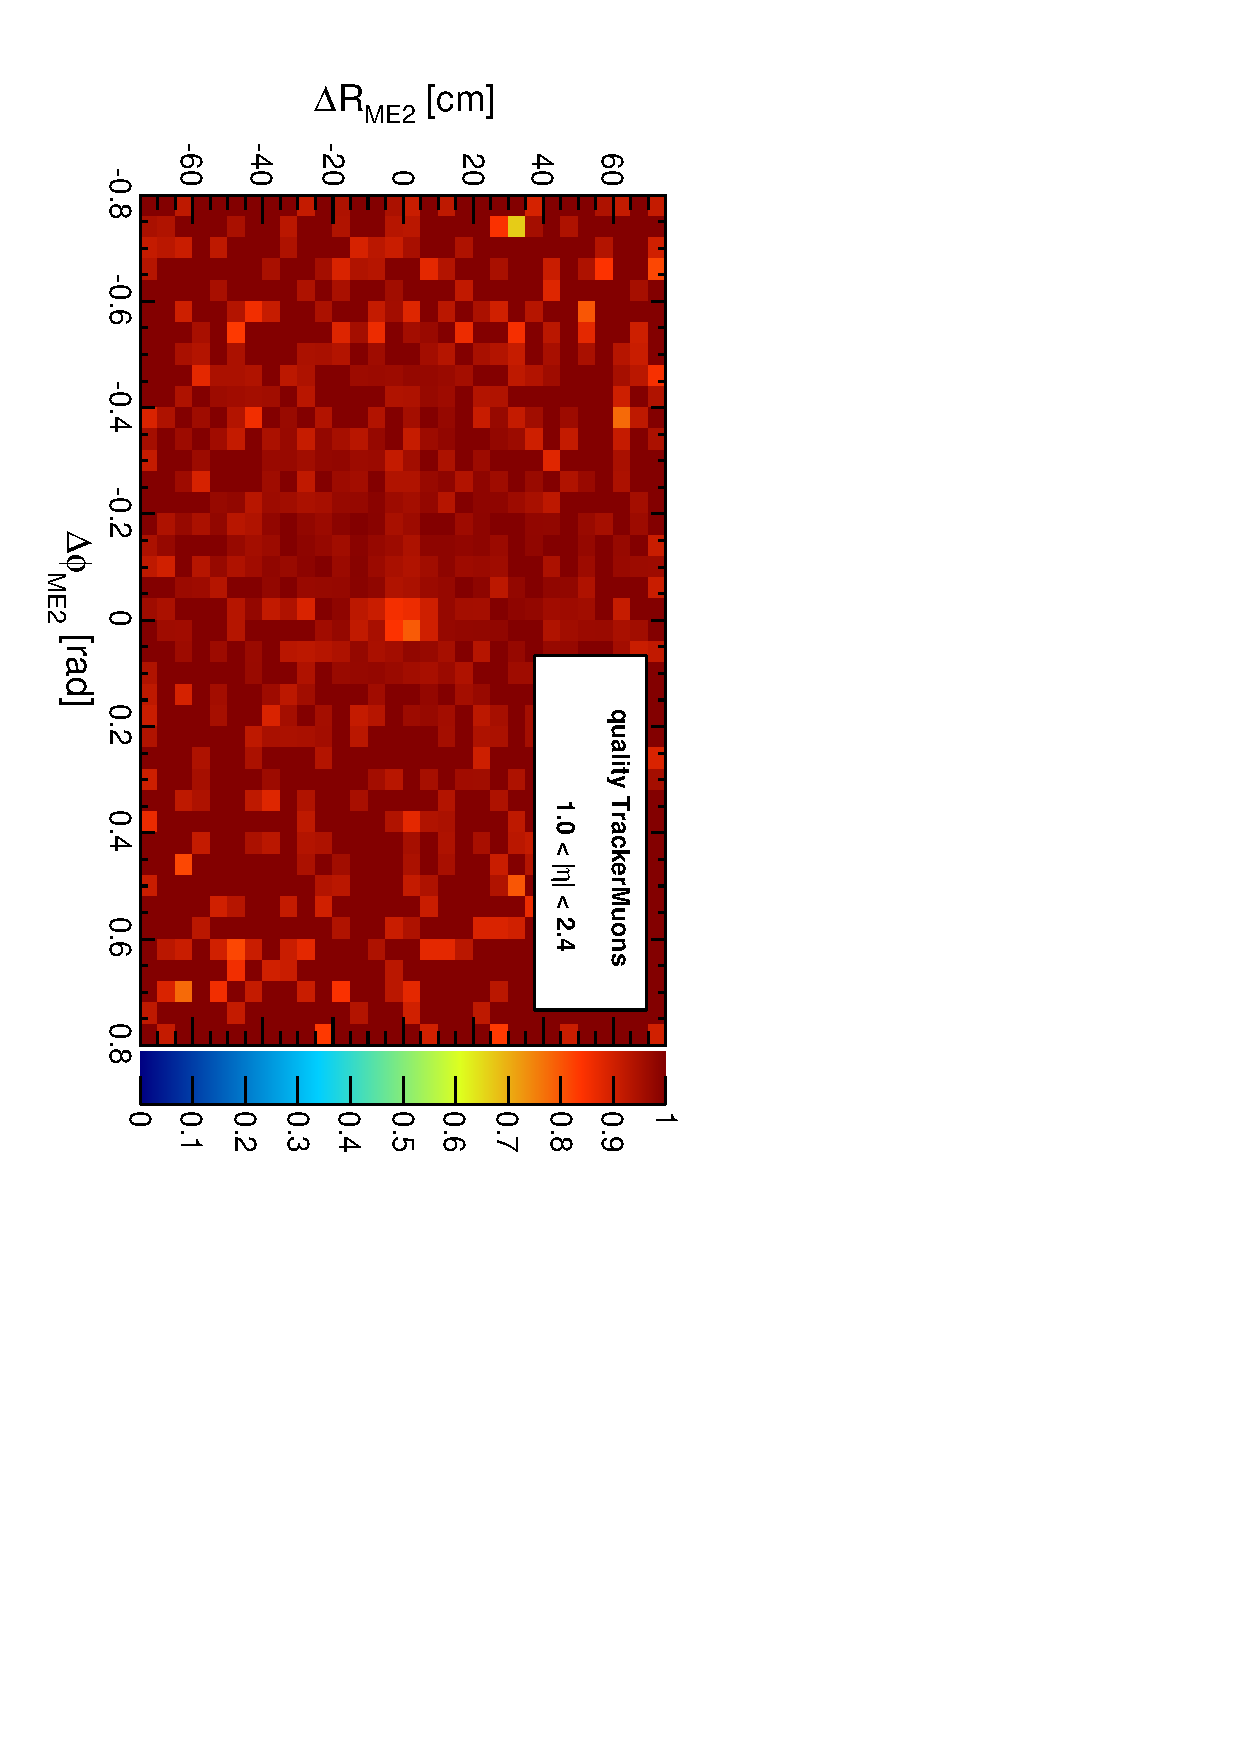
\includegraphics[height=0.49\linewidth, angle=90]{me2_PlainTrackerMuon.pdf}
\end{frame}

%% \begin{frame}
%% \frametitle{Outline}
%% \begin{itemize}\setlength{\itemsep}{0.75 cm}
%% \item 
%% \end{itemize}
%% %% \hspace{-0.83 cm} \textcolor{darkblue}{\Large Outline2}
%% \end{frame}

%% \section*{First section}
%% \begin{frame}
%% \begin{center}
%% \Huge \textcolor{blue}{First section}
%% \end{center}
%% \end{frame}

%% \begin{frame}
%% \end{frame}

\end{document}
